% !TEX root = as_grf_sopt.tex
\begin{figure*}[t]
\begin{center}
\begin{tabular}{c@{}c@{}c}
\subfigure[5000 Populated Places]{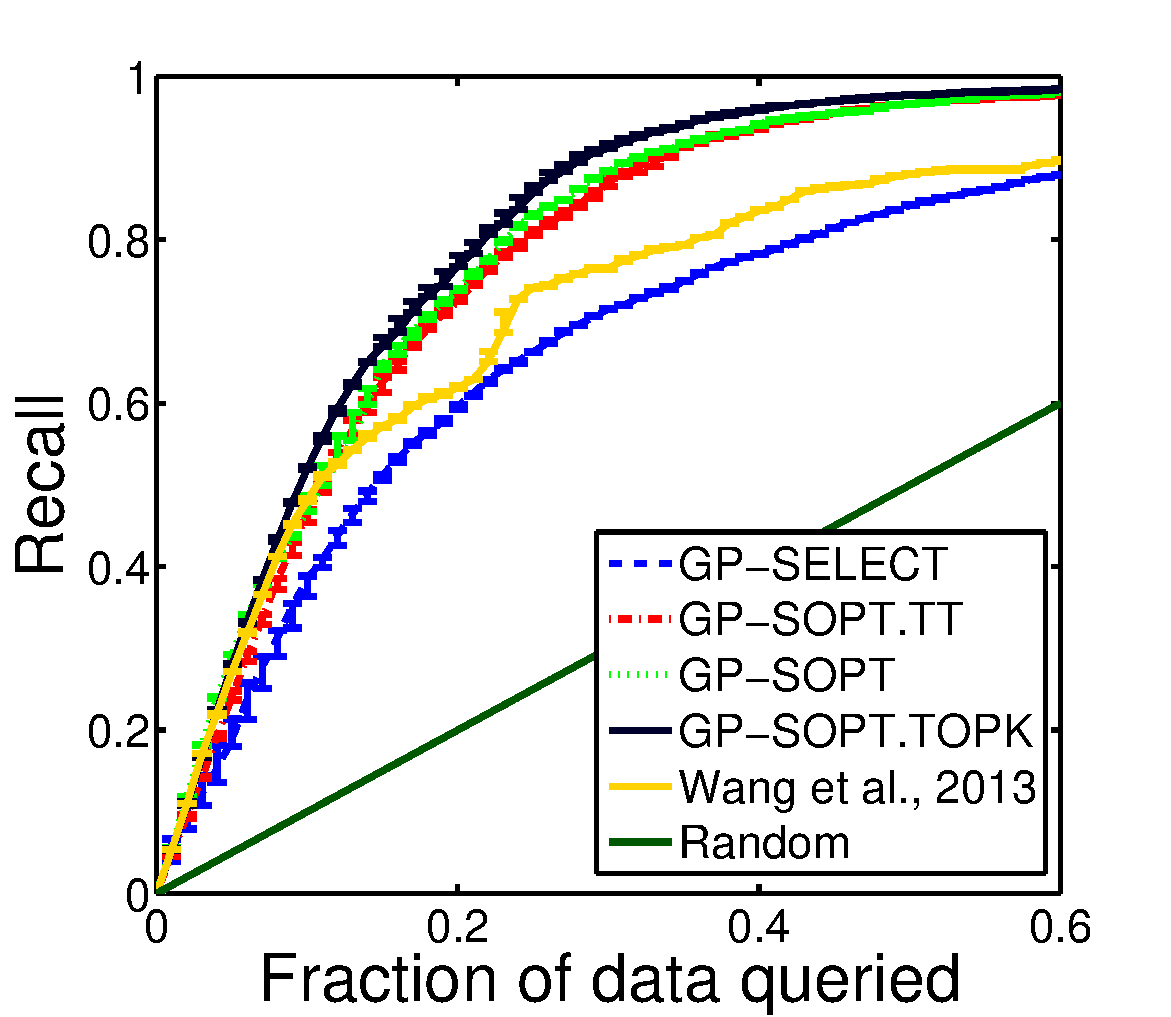
\includegraphics[width=0.31\textwidth,height=0.25\textwidth]{../exp/final_results/populated_places_5000_result_5seeds_top15p_omega0-001_lapnorm0_new.pdf}} &
\subfigure[Wikipedia]{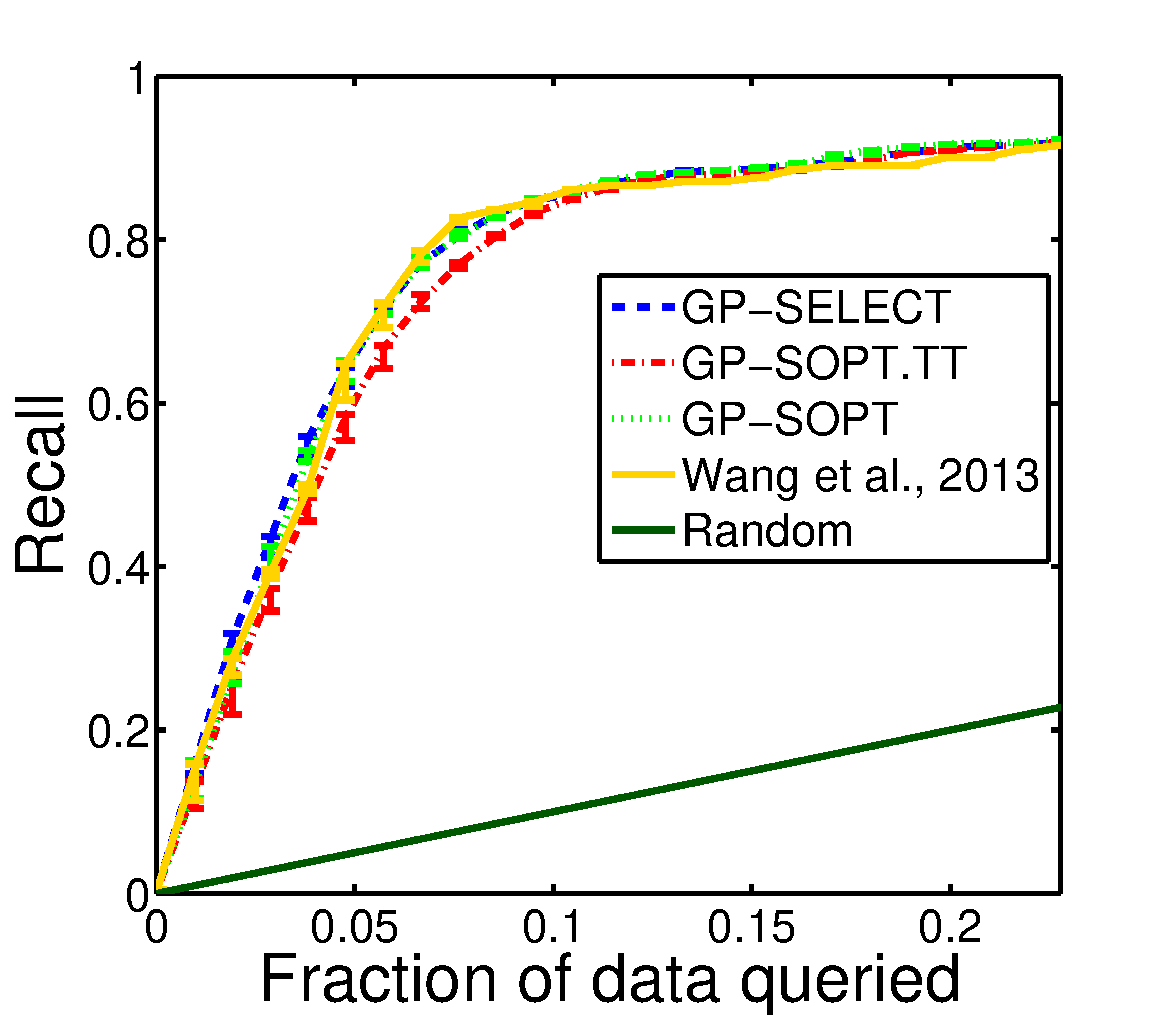
\includegraphics[width=0.31\textwidth,height=0.25\textwidth]{../exp/final_results/wiki_result_5seeds_top15p_omega0-001_lapnorm0_new.pdf}} &
\subfigure[Citation Network]{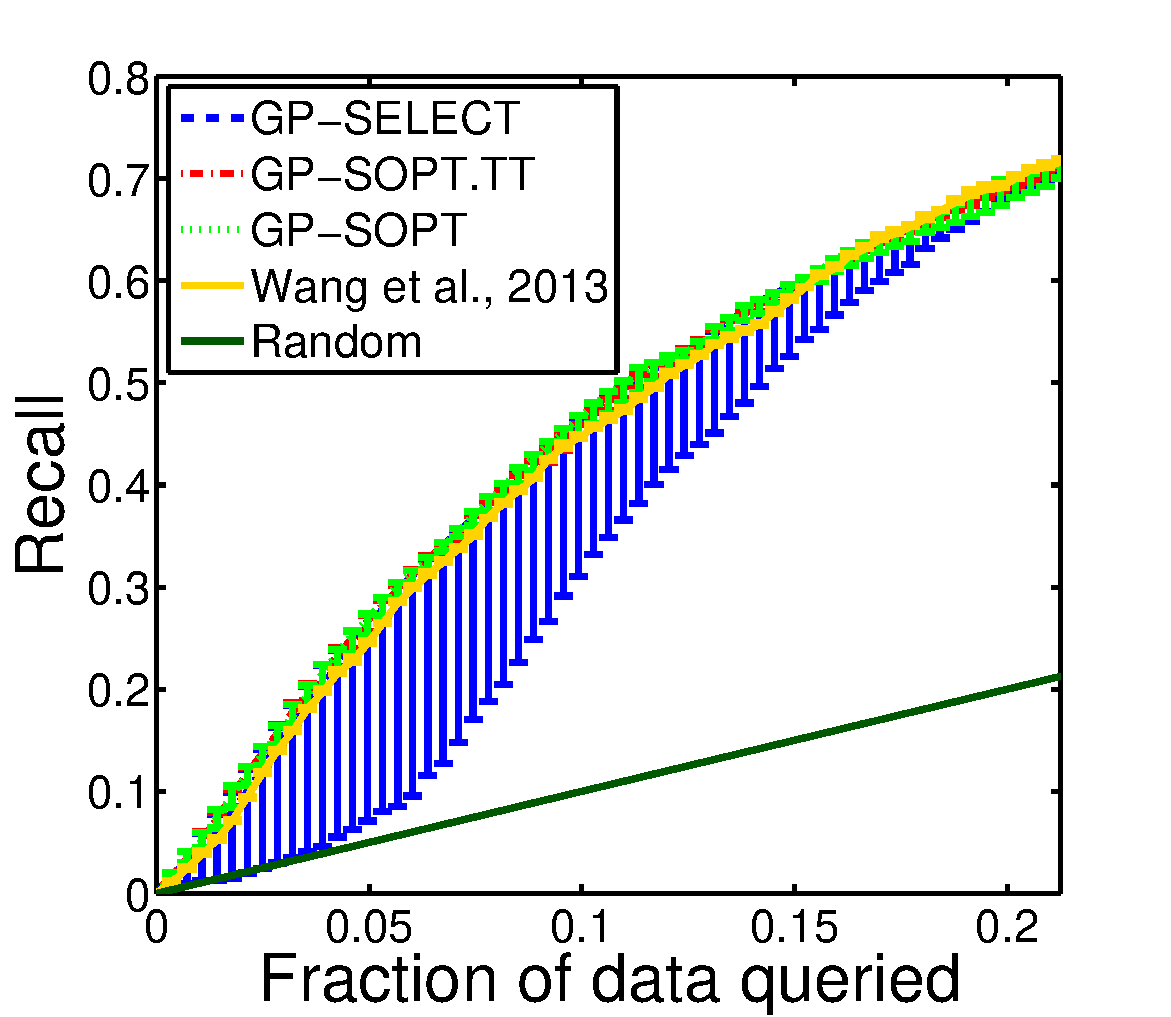
\includegraphics[width=0.31\textwidth,height=0.25\textwidth]{../exp/final_results/new_nips_result_5seeds_top15p_omega0-001_lapnorm0.pdf}}
\end{tabular}
\end{center}
\caption{Recall vs. fraction of data queried}
\label{fig:results}
\end{figure*}
We conduct experiments on three graph data sets that were studied by \cite{wang2013active}
and a version of the Enron e-mail data by \cite{enron}.
\subsection[Three Graph Datasets of Wang et al., 2003]{Three Graph Datasets of \cite{wang2013active}}
We briefly summarize the datasets below.

\textbf{5000 Populated Places.} The nodes of this graph are 5000 concepts in the DBpedia\footnote{www.dbpedia.org} ontology marked as populated places.
Each place is supported by a Wikipedia page, and an undirected edge is created between two 
places if either one of their two Wikipedia pages links to the other. There can be multiple 
edges between two places. The DBpedia 
ontology divides populated places into five categories: administrative regions, countries, cities, towns and villages.
The 725 administrative regions are selected as our target class while all the others are considered to be in null class.   
  
\textbf{Citation Network.} This dataset consists of 14,117 papers in top Computer Science venues available on citeseer. 
The graph is created by adding an undirected edge between two papers if either one cites the other. The 1844 NIPS papers
are chosen as our target class. 

\textbf{Wikipedia Pages on Programming Languages.} A total of 5,271 Wikipedia pages related to programming languages are the nodes 
of this graph, and an undirected edge exists between two pages if they are linked together. \cite{wang2013active} performed topic 
modeling and chose the 202 pages related to objective oriented programming as our target class.
%, treating all the others as null class.   
 
As demonstrated by \cite{wang2013active}, the three graphs and their target label distributions exhibit qualitative differences
and thus serve as good benchmarks. The citation network has many small components and target nodes appear in many of them, 
while the Wikipedia graph has large hubs and most target nodes reside in one of them. 
The graph of populated places lies in between these two extremes, with components of various sizes containing target nodes.   

On all of the three data sets we compare two of the proposed methods: GP-SOPT.TT and GP-SOPT against GP-SELECT (GP-UCB without replacement) 
and the active search algorithm (AS-on-Graph) by \cite{wang2013active}. We only evaluate GP-SOPT.TOPK on the 5000 populated places data
due to its heavy computation. For each dataset we perform 5 independent runs, each with a randomly
chosen target node as the warm start seed. 
For the proposed methods and GP-SELECT, the main tuning parameters  
are the exploration-exploitation trade-off parameter $\alpha_t$ and the observation noise variance $\sigma^2$.
For GP-SOPT.TT and GP-SOPT.TOPK there is additionally the thresholding parameter $k$. 
We consider the following values for them. 
Populated Places: $\alpha_t \in \{4,2,1,0.1,0.01,0.001\}$, $\sigma^2 \in \{1,0.5,0.25,0.1\}$ and $k \in \{200,400,800\}$. 
Wikipedia: $\alpha_t \in \{0.1,0.01,0.001\}$, $\sigma^2 \in \{1,0.5,0.25,0.1\}$ and $k \in \{200,400,800\}$.  
Citation Network: $\alpha_t \in \{1,10^{-1},10^{-2},10^{-3},10^{-4}\}, \sigma^2 \in \{1,0.5,0.25,0.1\}$ and  $k \in \{400,800,1600\}$.
Although in theory $\alpha_t$ should be iteration-dependent, we find that a fixed value often performs well in practice.
On all data sets we set the kernel regularization parameter $\omega_0 = 0.01$.
\cite{wang2013active} algorithm has several parameters, and we only tune the exploration-exploitation trade-off parameter $\alpha$. It is set to 0.1 on Populated Places and Citation Network,
and 0.0001 on Wikipedia, which are the best performing values. Other parameters are set based on \cite{wang2013active}. 


Results are in  Figure~\ref{fig:results}, where we plot the recall, i.e., the fraction of 
targets found by the algorithms, versus the fraction of the whole data set queried.
More specifically, for each algorithm we obtain its mean recall curve over the top 15\% (except for \cite{wang2013active})
parameter combinations in each experiment, as judged by the area under the recall curve.
We then plot the median, maximum and minimum over the five runs in Figure~\ref{fig:results}.

The three proposed methods clearly outperform \cite{wang2013active} and GP-SELECT on Populated Places, while all methods 
perform equally well on Wikipedia. We think this has to do with the underlying graph structure and target distribution.
As mentioned before, target nodes in the Populated Places graph are spread over sub-graphs of various sizes, and therefore exploration strategies 
do make a difference. We observe that the proposed methods tend to select high-degree nodes in the first few iterations, thereby
gaining much information, while GP-SELECT initially selects low-degree nodes.  
In contrast, most target nodes in the Wikipedia graph reside in one large component, and therefore 
less exploration is needed. In fact, the best values for $\alpha_t$ are very small, suggesting that an exploitation-only 
strategy is good enough for this data. On Citation Network, most methods perform well except that GP-SELECT performs 
quite poorly in one run. This may again indicate GP-SELECT is less robust against low-degree nodes. 
\subsection{Enron E-mails}
We experimented on the Enron e-mail data set\footnote{Available at \url{http://cis.jhu.edu/~parky/Enron/execs.email.linesnum.ldctopic} \label{note:enron}} 
with topics assigned by \cite{enron} based on the annotations by \cite{enron_topics}. 
We further processed the dataset into a format suitable for active search experiments as detailed below. 
Each e-mail $i$ is represented by a unique Unix time stamp $t_i$, a unique sender index and the set of receiver (excluding self-copying) indices, which are collectively 
denoted as $U_i$. Between e-mails $i$ and $j$, we created an edge with the following weight:

\centerline{
$A_{ij} :=  \exp\left( - (t_i - t_j)^2 / \tau^2 \right) \cdot |U_i \cap U_j| / \sqrt{|U_i||U_j|}$,	
}

where $\tau = 12$ weeks in seconds and $|U_i|$ denotes the size of $U_i$. 
We thus measure pairwise similarity among e-mails by the product of 
nearness in time and degree of overlap between users involved. 
The resulting e-mail graph has 20,112 nodes, and we chose the subset of 803 e-mails that are assigned topic 16 in LDC topics\footnoteref{note:enron}, 
which is related to the downfall of Enron, to be the target class in this experiment.

Due to the size of the dataset, we only compared three methods: GP-SOPT.TT, GP-SELECT and \cite{wang2013active}
in three independent runs each initialized with a target node chosen uniformly at random.
We also limited the tuning parameters to be the following fixed values across the three runs:
$(k,\alpha,\sigma^2,\omega_0) = (800, 0.001, 0.05, 0.01)$ for GP-SOPT.TT, $(\alpha, \sigma^2, \omega_0) = (0.01, 0.05, 0.01)$ for GP-SELECT, 
and $\alpha = 0.001$ for \cite{wang2013active}. These values were chosen based on a coarse parameter search to be indicative of the performance of each method on this data set.
\begin{figure}[t]
\centering
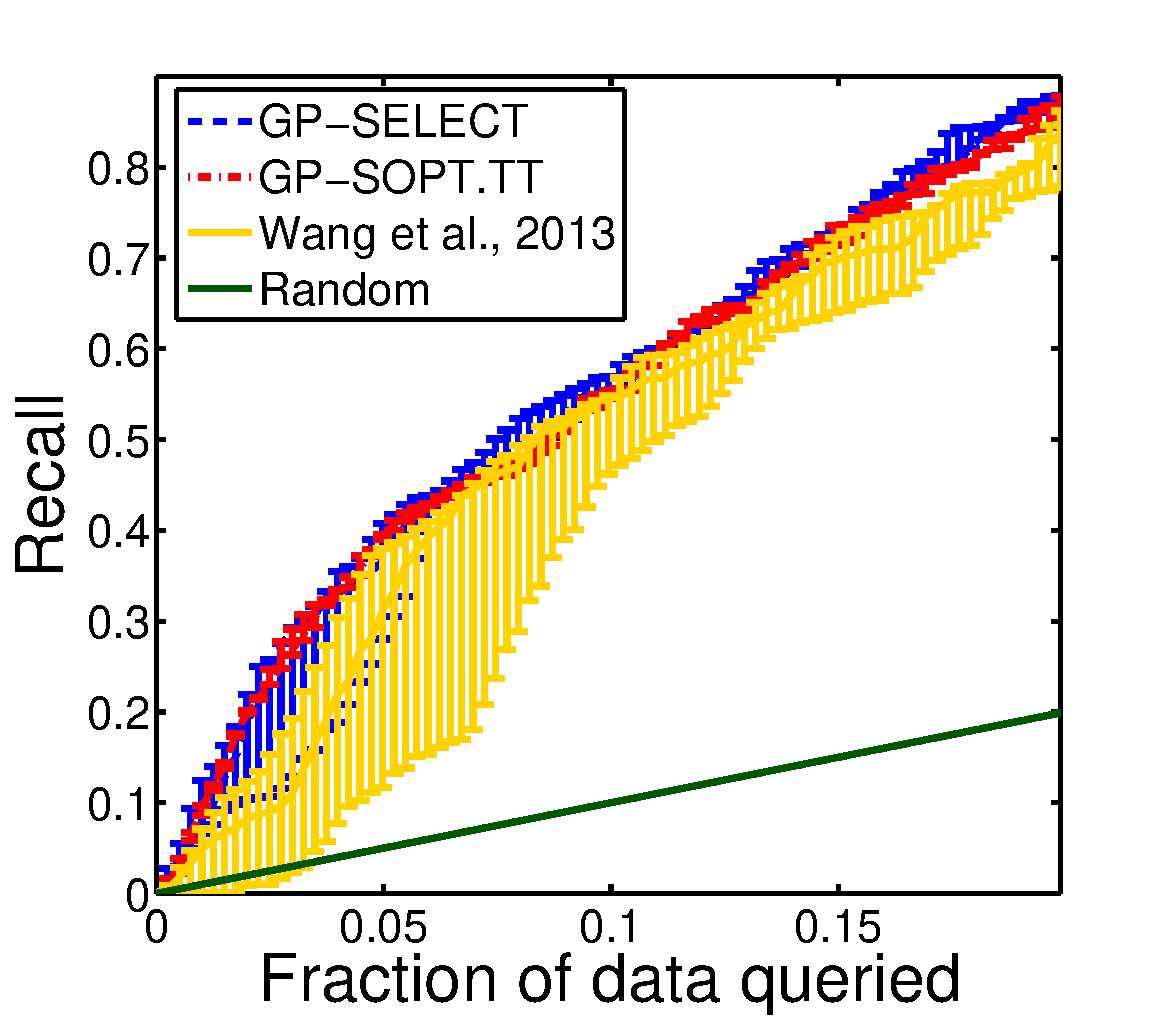
\includegraphics[width=0.31\textwidth,height=0.25\textwidth]{../exp/final_results/enron.pdf}
\caption{Enron: recall vs. fraction of data queried}
\label{fig:enron}
\end{figure}
Results are in Figure~\ref{fig:enron}, which shows GP-SOPT.TT is more stable across initial seeds than the other methods, and outperforms \cite{wang2013active} significantly at early iterations. 
